\documentclass{ReportTemplate}
\usepackage{titlesec}
\usepackage[francais]{babel}
\usepackage[T1]{fontenc}
\title{CSEL}
\author{Macherel Rémy}
\date{\today}
\subtitle{Rapports des TP}
\subsubtitle{Git du projet : \href{https://github.com/Mathistis/csel-workspace}{https://github.com/Mathistis/csel-workspace}}
\location{Fribourg,}
\contact{remy.macherel@master.hes-so.ch}
\version{1.0}
\titlespacing*{\chapter}{0pt}{-60pt}{20pt}
\begin{document}

\maketitlepage

\newpage

\maketableofcontent

\medskip

\titleformat{\chapter}[display]
    {\Huge\bfseries}
    {}
    {0pt}
    {\thechapter.\ }
    

\chapter{Introduction}
Ce rapport décrit l'architecture ainsi que le développement et les
fonctionnalités du mini-projet réalisé lors du cours \textit{MA-CSEL} suivi lors
du semestre de printemps 2022 du master MSE. Ce projet consiste à mettre en
pratique les notions vues dans le cours par l'intermédiaire de l'implémentation
d'un gestionnaire de ventilateur pour le processeur de la cible. Notre cible
n'ayant pas de réel ventilateur, son fonctionnement sera simulé par le
clignotement d'une LED symbolisant la fréquence de celui-ci ainsi qu'un écran
OLED affichant quelques valeurs importantes.\newline
Le but du travail est donc de concevoir une application permettant de simuler la
gestion de la vitesse de rotation d'un ventilateur en fonction de la température
du processeur. Les fonctionnalités suivantes seront donc implémentées:
\begin{itemize}
    \item Supervision de la température du processeur et la gestion de la
    vitesse de clignotement de la LED à l'aide d'un module noyau.
    \item Un daemon en espace utilisateur qui offrira des services pour une
    gestion manuelle et prendra en compte la gestion des appuis sur les boutons
    afin d'augmenter la vitesse de rotation, de la diminuer et de passer du mode
    manuel à automatique.\newline
    Ce daemon pourra également, à l'aide d'une interface IPC, communiquer avec
    une application de type \textit{CLI} pour la gestion du clignotement et du
    mode.
    \item Une application \textit{CLI} pour piloter le système via l'interface IPC.
\end{itemize}

\chapter{Architecture logicielle}
\begin{figure}[H]
    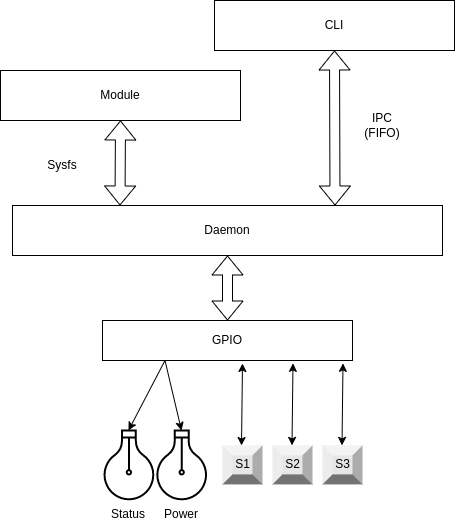
\includegraphics[width= \textwidth]{imageSources/Diagramme_Fonctions.drawio.png}
    \caption{Diagramme de principe de l'application}
    \label{fig:functionDiagram}
\end{figure}
\chapter{Conception du module}
Ce chapitre traite du développement du module noyau permettant de surveiller la
température du processeur ainsi que la gestion du clignotement de la LED status.
Ce module est dans le répertoire class et est composé de deux attributs:
\begin{itemize}
    \item is\_manu
    \item freq
\end{itemize}
Ces deux attributs sont représentés dans le userspace par des fichiers du sysfs.
Le but de ce module est de faire clignoter la LED en mode automatique (si
is\_manu est à 0) ou en mode manuel (si is\_manu est à 1). Le module implémente
un timer (\textit{<linux/timer.h>}) (voir fichiers \textit{timer\_controller.h
et .c}) qui est créé avec une fonction à exécuter à
chaque fois que son décompte est terminé. Lorsque le temps est écoulé, le
programme vérifie le mode actuel grâce à l'attribut \textit{is\_manu} et si le
mode actuel est manuel, il va regarder la fréquence inscrite dans le fichier
\textit{freq} puis calculer le prochain \textit{jiffies} correspondant à la
période de la fréquence de la manière suivante :
\usemintedstyle{vs}
\begin{minted}[linenos=False,frame=none]{c}
#define NEXT_JIFFIE_FROM_FREQ(freq) (jiffies + (HZ / freq))
\end{minted}
Il va ensuite changer l'état de la LED et réamorcer le timer.\newline
Pour le mode automatique, il va simplement lire la température du
microprocesseur et obtenir la fréquence correspondante (voir figure
\ref{fig:ledFrequencies}), puis écrire cette valeur dans le fichier freq et
réamorcer le timer.
\begin{figure}[H]
    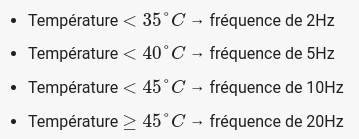
\includegraphics[width= \textwidth]{imageSources/Led_Frequencies.png}
    \caption{Fréquences pour la led en mode automatique}
    \label{fig:ledFrequencies}
\end{figure}
Dans le module, nous avons séparé les codes en deux parties, un fichier
\textit{controller.c} (avec son .h dédié) qui représente une bibliothèque
permettant la gestion des modes du programme. Ce controller permet d'initialiser
les différents éléments utilisés dans le module (comme gpio, capteur de
température, timers, etc.), il sert en quelque sorte d'interface de gestion des
éléments du module noyau.\newline
Le deuxième fichier \textit{gpio.c} (également accompagné de son .h) permet quand à lui la gestion
des gpio ainsi que leur initialisation.\newline
Un autre code présent dans l'utilisation du module est le
\textit{temp\_controller}, celui-ci permet à l'aide de la bibliothèque
\textit{linux/thermal.h} de récupérer la température actuelle du
processeur.\newline
Dans le fichier \textit{skeleton.c} (en quelques sorte le main du module), nous
appelons la fonction \textit{init\_controller} qui va permettre l'initialisation
des gpio, du timer ainsi que de la lecture de la température.\newline
Ce module va également créer et initialiser dans le sysfs les fichiers
nécessaires à la transmission de nos informations.\newline
Notre module étant de type \textit{class} il possède des attributs qui seront
stocké dans le sysfs sous \textit{/sys/class/<mod\_name/...} et lors de la
déclaration des attributs du module (voir figure \ref{fig:sysfsInit}), on
définit deux variables statiques au module ainsi que deux méthodes de lecture et
écriture qui permettront de gérer ces deux fichiers.
\begin{figure}[H]
    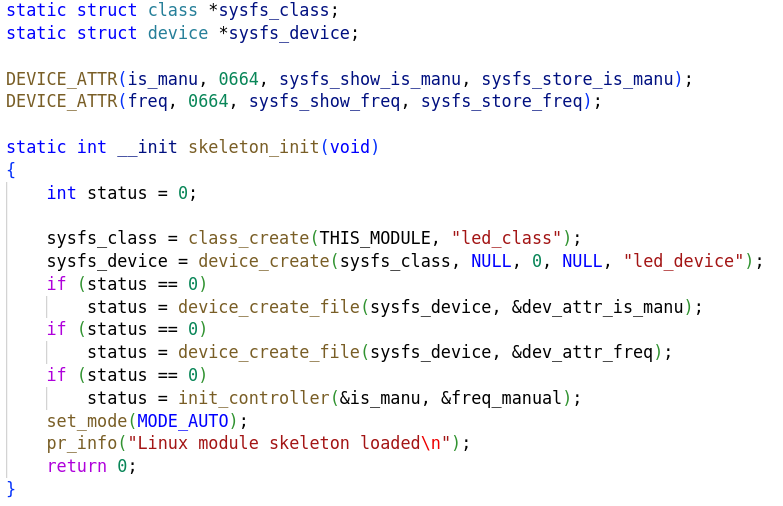
\includegraphics[width= \textwidth]{imageSources/Skeleton_Init.png}
    \caption{Création des fichiers nécessaires dans le sysfs}
    \label{fig:sysfsInit}
\end{figure}
Dans l'initialisation du module (figure \ref{fig:sysfsInit}), on se charge également de créer le device pour
le sysfs ainsi que les différents fichier qui nous servirons pour lire et écrire
nos valeurs.\newpage
Nous avons également dans ce module déclaré quelque fonctions permettant la
lecture ainsi que l'écriture des fichiers dans le sysfs.
\begin{figure}[H]
    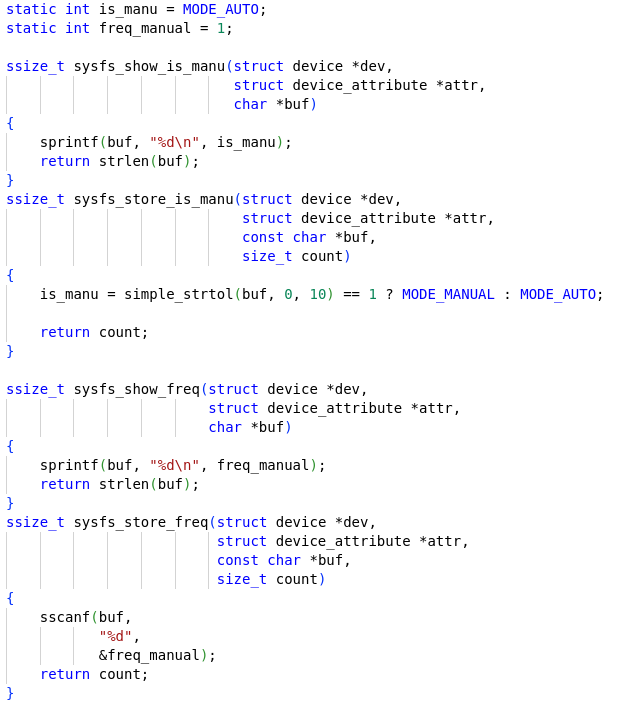
\includegraphics[width= \textwidth]{imageSources/Utility_Fct_Module.png}
    \caption{Fonctions de lecture/écriture des fichiers du sysfs}
    \label{fig:sysfsFunctions}
\end{figure}
On observe dans la figure \ref{fig:sysfsFunctions} que ces fonctions permettent
de lire et écrire les différents fichiers correspondant par exemple au mode
manuel ou l'affichage de la fréquence.\newpage
\section{Difficultés rencontrées sur le module}
Nous avons eu quelques soucis à fournir au début un code clair et bien séparé
c'est pourquoi nous avons opté pour la solution des controllers ainsi que des
fichiers séparés.\newline
Une autre difficulté fût de bien comprendre que \textit{DEVICE\_ATTR} est en
réalité une macro qui permet de créer plein de choses différentes concernant les
fichiers du sysfs et au premier abord nous n'avions pas pleinement conscience de
cela et avons eu un peu de peine à mettre en place ceci.
\chapter{Conception du daemon}
Ce chapitre traite du développement du deamon offrant les services permettant la
gestion de la fréquence ainsi que le choix du mode.

\end{document}


